\documentclass[11pt]{article}

\usepackage{xcolor}
\usepackage{listings}
\usepackage{graphicx}
\usepackage{subfigure}
\lstset{ %
language=C++,                % choose the language of the code
basicstyle=\footnotesize,       % the size of the fonts that are used for the code
backgroundcolor=\color{white!3!white},  % choose the background color. You must add \usepackage{color}
showspaces=false,               % show spaces adding particular underscores
showstringspaces=false,         % underline spaces within strings
showtabs=false,                 % show tabs within strings adding particular underscores
frame=single,           % adds a frame around the code
tabsize=2,          % sets default tabsize to 2 spaces
captionpos=b,           % sets the caption-position to bottom
breaklines=true,        % sets automatic line breaking
breakatwhitespace=false,    % sets if automatic breaks should only happen at whitespace
escapeinside={\%*}{*)},          % if you want to add a comment within your code
  basicstyle=\footnotesize\ttfamily,
  keywordstyle=\bfseries\color{green!40!black},
  commentstyle=\itshape\color{gray!80!black},
  identifierstyle=\color{black},
}


\title{\textbf{Projet Proposal for 	 \\ Parametrized String Matching Implementation for Software Plagiarism Check}}

\author{
		\vspace{ 2 mm}\\
		Supervised By : \textbf{Prof. Srinivasaraghavan G}\\
		\vspace {2mm}\\
		\textbf{Team} \\	
		amit.tomar \\
		(MT2013008) \\
		\vspace{ -1 mm}\\		
		siddhesh.dosi\\								     
		(MT2013150) \\		
		\vspace{ -1 mm}\\					
		srinivas.r.vaidya\\
		(MT2013152) \\
		\vspace{ -2 mm}\\		
		\textbf{@iiitb.org}}
		
\date{29 - March - 2014}

\begin{document}
\lstset{language=C} 
\maketitle

\vspace{ 100 mm}

\section{Introduction}

This project aims at developing a Parametrized String Matching Implementation for Software Plagiarism Check, that given a collection of files which contain code in some programming language, will show a set of possible duplications of parts of the code among these. Comparing pieces of software will require discounting comments (optional and language dependent), extra/blank lines and spaces, variable renaming etc. The theory of parametrized string matching will be used to implementat this project. System will have an easy-to-use UI for selecting files/folders and shall report the plagiarism related information (matches found) in the UI in a nice manner.

\section{ Functional Requirements}

  \begin{center}
    \begin{tabular}{ | l | p{10cm} |}
    \hline
    {\textbf{Requirement.No.}} & {1.1} \\ \hline
    \textbf{Input}      & File option \\ \hline
    \textbf{Output}     & User prompted to select files from multiple folder. \\ \hline
    \textbf{Processing} & Populate the folder structure of file system. \\ \hline
    \end{tabular}
\end{center}

  \begin{center}
    \begin{tabular}{ | l | p{10cm} |}
    \hline
    {\textbf{Requirement.No.}} & {1.2} \\ \hline
    \textbf{Input}      & Browsing and selection of files and next button \\ \hline
    \textbf{Output}     & User is promted to enter code snippet to be ignored while processing \\ \hline
    \textbf{Processing} & File path validation \\ \hline
    \end{tabular}
\end{center}

  \begin{center}
    \begin{tabular}{ | l | p{10cm} |}
    \hline
    {\textbf{Requirement.No.}} & {1.3} \\ \hline
    \textbf{Input}      & Check plagiarism \\ \hline
    \textbf{Output}     & Plagiarism related log is generated.  \\ \hline
    \textbf{Processing} & Generate parameterized suffix tree to check amount of plagiarism. \\ \hline
    \end{tabular}
\end{center}

  \begin{center}
    \begin{tabular}{ | l | p{10cm} |}
    \hline
    {\textbf{Requirement.No.}} & {2.1} \\ \hline
    \textbf{Input}      & Folder option \\ \hline
    \textbf{Output}     & User is prompted to select Folder. \\ \hline
    \textbf{Processing} & Search for all the files in the selected folder and populate a list. \\ \hline
    \end{tabular}
\end{center}

  \begin{center}
    \begin{tabular}{ | l | p{10cm} |}
    \hline
    {\textbf{Requirement.No.}} & {2.2} \\ \hline
    \textbf{Input}      & Selection/Deselection of files from the populates list and next button \\ \hline
    \textbf{Output}     & User is promted to enter code snippet to be ignored while processing \\ \hline
    \textbf{Processing} & File path validation \\ \hline
    \end{tabular}
\end{center}

  \begin{center}
    \begin{tabular}{ | l | p{10cm} |}
    \hline
    {\textbf{Requirement.No.}} & {2.3} \\ \hline
    \textbf{Input}      & Check plagiarism \\ \hline
    \textbf{Output}     & Plagiarism related log is generated.  \\ \hline
    \textbf{Processing} & Generate parameterized suffix tree to check amount of plagiarism. \\ \hline
    \end{tabular}
\end{center}                    

\section{ Non - Functional Requirements}

External interface requirements : 

 \begin{enumerate}
 \item Shall be portable, across various hardware and software platforms.
\item Shall be scalable and reliable.
\item Shall be easy to use.
      
 \end{enumerate}

Performance requirements :

 \begin{enumerate}

\item Shall have a good response time.
 
  \end{enumerate}
  
\section{Goals of implementation}

Plagiarism is a serious issue in computer
science courses involving assessment of programming
assignments [1]. Being electronic in nature, it is very easy to copy code and it is difficult to differentiate between the original and copied work. Thus, there is a need for a tool to detect plagiarism 
automatically, assisting professor to check for any kind of copying done by students.

\section {UI Flow}

Following screen shots show the various UI screens :

\begin{figure}
\hfill
\subfigure[Starting screen]{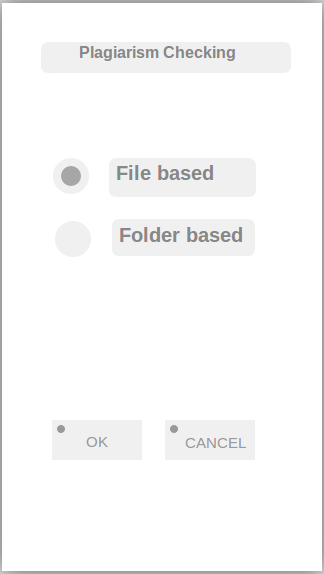
\includegraphics[width=6cm]{Screen1}}
\hfill
\subfigure[Screen to select file]{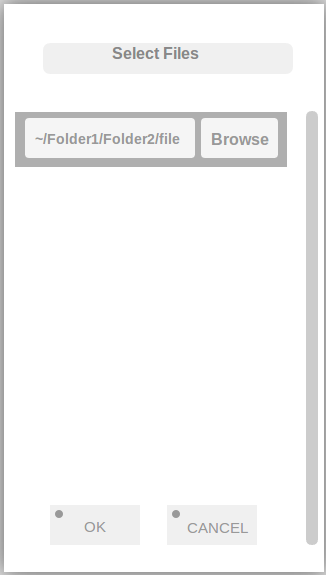
\includegraphics[width=6cm]{Screen2}}
\hfill

\end{figure}

\begin{figure}
\hfill
\subfigure[Screen to select/deselect file]{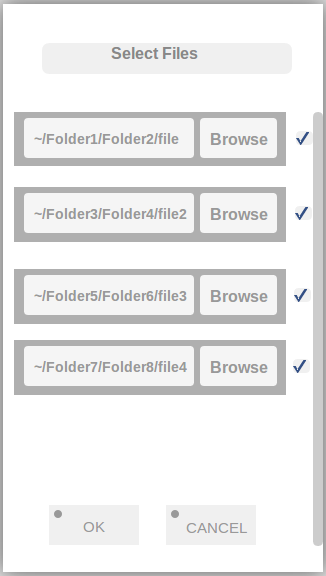
\includegraphics[width=6cm]{Screen3}}
\hfill
\subfigure[Screen to display all the files in the selected folder]{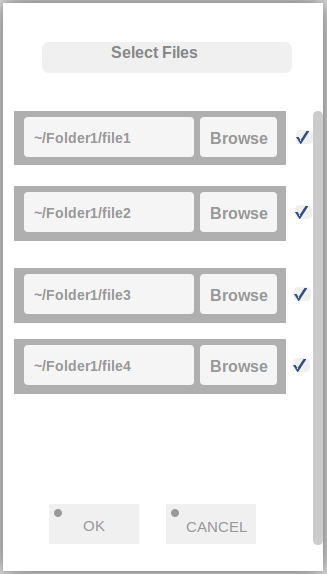
\includegraphics[width=6cm]{Screen4}}
\hfill

\end{figure}

\begin{figure}
\hfill
\subfigure[Screen to select code snippet]{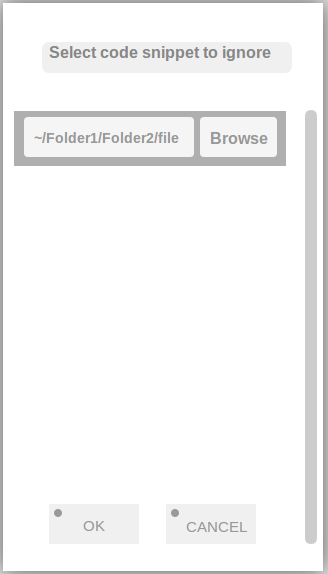
\includegraphics[width=6cm]{Screen5}}
\hfill
\subfigure[Screen to display plagiarism analysis report]{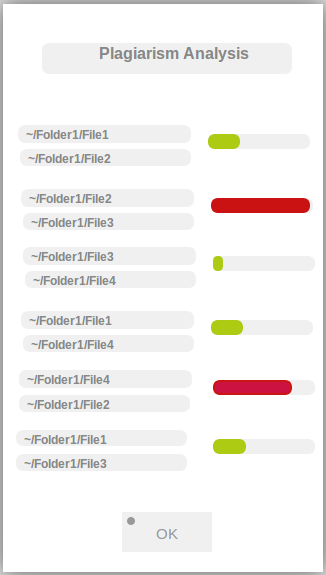
\includegraphics[width=6cm]{Screen6}}
\hfill

\end{figure}

\begin{figure}[h!]

  \centering
    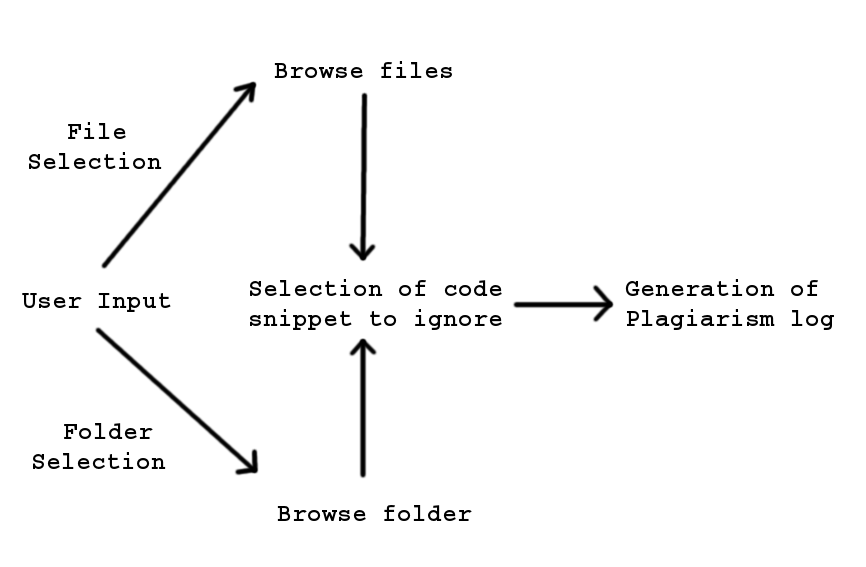
\includegraphics[width=1.2\textwidth]{DecisionTree}
      \caption{Decision Tree}
\end{figure}

\section{Project deliverables and estimated time}

\begin{enumerate}
  \item \textbf{Milestones}
  \begin{enumerate}
    \item \textbf{Requirement Specification} :  \\
    Date of submission : 7 - Feb - 2014 \\ 
    (Already submitted to Prof. Srinivasraghvan)\\
    \item \textbf{Literature Survey} : \\
Expected date of completion : 15 - April - 2014 \\ 
Expected time : 40 Hours\\
    \item \textbf{Building suffix tree data structure} :\\
    Expected date of completion : 15 - May - 2014 \\ 
    Expected time : 30 Hours\\
    \item \textbf{Identifying duplicate code using suffix tree}: \\
    Expected date of completion : 1 - June - 2014 \\ 
    Expected time : 25 Hours\\
    \item \textbf{Implementation of UI}: \\
    Expected date of completion : 10 - June - 2014 \\ 
    Expected time : 10 Hours\\
    \item \textbf{Parameterized implementation for software plagiarism check}:\\
    Expected date of completion : 1 - July - 2014 \\ 
    Expected time : 40 Hours\\
    \item \textbf{Integration of UI with parameterized string matching code}:\\
    Expected date of completion : 15 - July - 2014 \\ 
    Expected time : 20 Hours\\
    \item \textbf{Testing}:\\
    Expected date of completion : 31 - July - 2014 \\ 
    Expected time : 20 Hours\\
           
  \end{enumerate}
  \item \textbf{List of final deliverables}:
    \begin{enumerate}
  \item Requirement specification document.
  \item Design document.
  \item User manual.
  \item Deployment manual.
    \end{enumerate}

\end{enumerate}


\section{Hardware and Software requirements}

\begin{center}
    \begin{tabular}{ | l | l | l | p{6cm} |}
    \hline
    \textbf{S.No.} & \textbf{Software} & \textbf{Version} & \textbf{Purpose}\\ \hline
    1 & Ubuntu Linux & 13.04 & Operating system. \\ \hline
    2 & GitHub & 1.8.3.2 &Version Control \\ \hline
    3 & Spyder & 2.2.1 & IDE for Python \\ \hline
    4 & GIMP & 2.6 & Image editing for documentation \\ \hline
    5 & Gummi & 0.6.5 & LaTeX editing for documentation \\ \hline    

    \end{tabular}
\end{center}

\section {Coding guidelines}	

  \begin{enumerate}
  
\item \textbf{Class} \\
All class names should begin with capital letter, with all subsequent words beginning with a capital letter 
too.\\
\textbf{eg.} \\
class ThisIsAClassName{}\\  
class Administration{}\\
class FooClass {}\\

\item \textbf{Function}\\
All function names should begin with a small letter, with all subsequent words beginning with a capital  
letter.\\
\emph{eg.}\\
void thisIsAFunction( void );\\
int fooFunction ( string ) ;\\

Names representing methods or functions must be verbs.
eg.\\
int getSystemVolume( void ) ;\\
void setSytemContrast( int ) ;\\
char findFirstCharacter( void ) ;\\

\item \textbf{Variables}\\
All primitive data type variables must begin with the first character of data type in small followed by the 
name of variable starting with a capital letter. Subsequent words will have their first character capital.\\
\textbf{eg.}\\
dataType dThisIsAVariableName\\
int          iSystemVolume; \\
char       cAnAlphabet;\\
float       fCurrentMonthSalary;\\
long       lVolumeOfWater;\\
double   dTotalTtax;\\
string     sMyName;\\
bool       bIsSet;\\

Use of global variables should be avoided as far as possible.

\item \textbf{Objects of class}
All object names must begin with ''obj'' followed by the exact class name.\\
\textbf{eg.} \\
FooClass objFooClass;\\
In   case   multiple   instances   of  a   class   are   to   be   used,   above   described   name   is   to   be   followed   by   some information about the object. All these subsequent words must begin with a capital letter. \\
\textbf{eg.} \\
Employee objEmployeeAmit;\\
Employee objEmployeeHemant;\\
Employee objEmployeeKaustubh;\\

\item \textbf{Pointer types}\\ 
If a variable is of pointer type, then its name should be preceded by ''ptr\_''\\
\textbf{eg}.\\
int * ptr\_iSalary;\\
char * ptr\_cNewCharacter;\\
FooClass * ptr\_objFooClassMemory;\\

\item \textbf{Array type}
All array names should be preceded by ''arr\_''\\
\textbf{eg.}\\
int arr\_iSalary [ 10 ];\\
char arr\_cNewCharacter [ 200 ] ;\\
FooClass arr\_objFooClassMemory [ 5 ] ;\\

\item {\textbf{List type}}\\
All list names should be preceded by ''lst\_''\\
\textbf{eg.}\\
list[int] lst\_iRollNumber;

  \end{enumerate}

\begin{thebibliography}{1}

\bibitem PPeter Vamplew, Julian Dermoudy, "An Anti-Plagiarism Editor for Software Development Courses", \emph{Proceeding
ACE '05 Proceedings of the 7th Australasian conference on Computing education - Volume 42
Pages 83-90 }, 2005.

\bibitem EE.M. McCreight "A space-economical suffix-tree
construction algorithm", J. ACM 23,2 (1976), pp. 262-272.

\bibitem BBrenda S. Baker, "A Program for Identifying Duplicated Code, Computing Science and
Statistics" 24 (1992), Interface Foundation of North America, pp. 49-57

\bibitem BBrenda S. Baker, "Parameterized Duplication in Strings: Algorithms and an Application to Software Maintenance", SIAM Journal on Computing.

\end{thebibliography}

\end{document}

